\documentclass{beamer}
\usepackage[utf8]{inputenc}
\usepackage{listings}
\usetheme{Warsaw}
\title[Network layer design in Android]{Android\\Network layer design}
\author{Santiago Munín}
\institute{Universidade da Coruña}
\date{May, 2013}
\begin{document}

\begin{frame}
\titlepage
\end{frame}

\section{Introduction}
\begin{frame}{Motivation}
\begin{itemize}
\item A huge number of successful mobile applications use an Client/Server architecture.
\item These architectures use the network as a tool to communicate.
\item {\bf Examples}: Twitter, Facebook, 4square, Evernote...
\end{itemize}
\end{frame}

\begin{frame}{Client/Server architecture}
\begin{itemize}
\item Communications are usually performed through HTTP (or HTTPS) with servers (usually REST servers).
\item Markup languages (such as JSON or XML) are used in order to exchange information between nodes.
\item These are costly communications$\rightarrow$ They have to be done through another thread or they would block the UI (decreasing the user experience).
\item Simple solution: the network operation should be excuted in background and use the UI thread only after getting the response without blocking it (a loading dialog could be showed meanwhile).
\end{itemize}
\end{frame}

\begin{frame}{AsyncTask}
\begin{itemize}
\item Android provides us with a class which wraps the thread handling.
\item AsyncTask allows us to execute a task in background and use the result in foreground without blocking the UI.
\item {\bf More information}: \url{http://developer.android.com/reference/android/os/AsyncTask.html}
\end{itemize}
\end{frame}

\section{First design: naive approach}
\subsection{Class diagram}
\begin{frame}{Class diagram}
\begin{figure}
\begin{center}
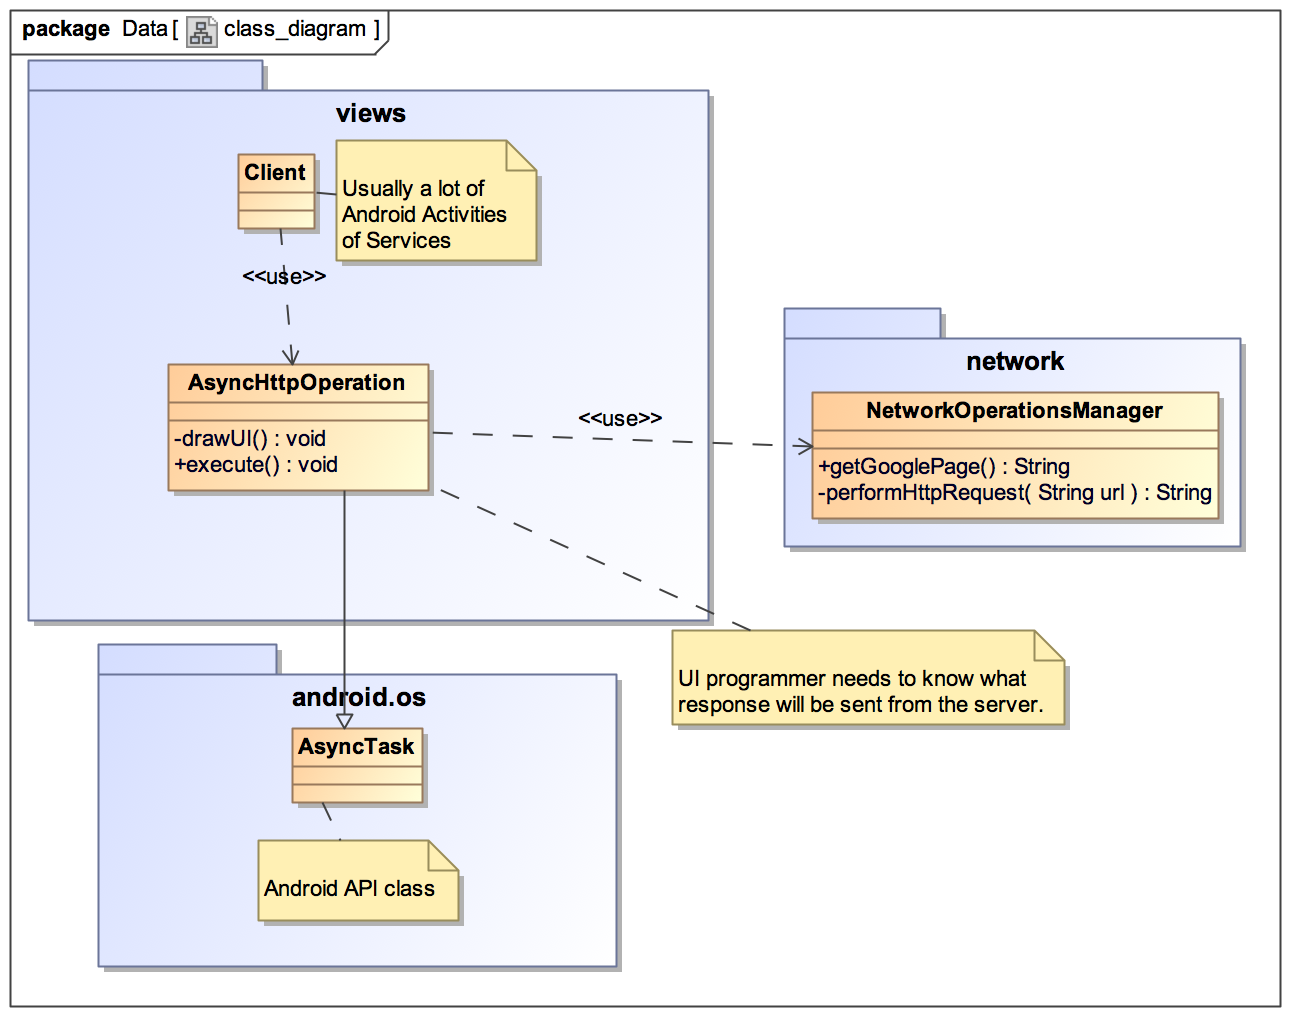
\includegraphics[scale=0.6]{../naive/design_models/class_diagram}
\end{center}
\end{figure}
\end{frame}

\begin{frame}{Explanation}
\begin{itemize}
\item The client (usually ``Activities'' Android) uses classes which inherit from ``AsyncTask'' in order to not block the UI.
\item The ``NetworkOperationsManager'' class contains all the logic relative to the network calls (url, parameters). It may be responsible of the response parsing and caching.
\end{itemize}
\end{frame}

\subsection{Sequence diagram}
\begin{frame}{Sequence diagram}
\begin{figure}
\begin{center}
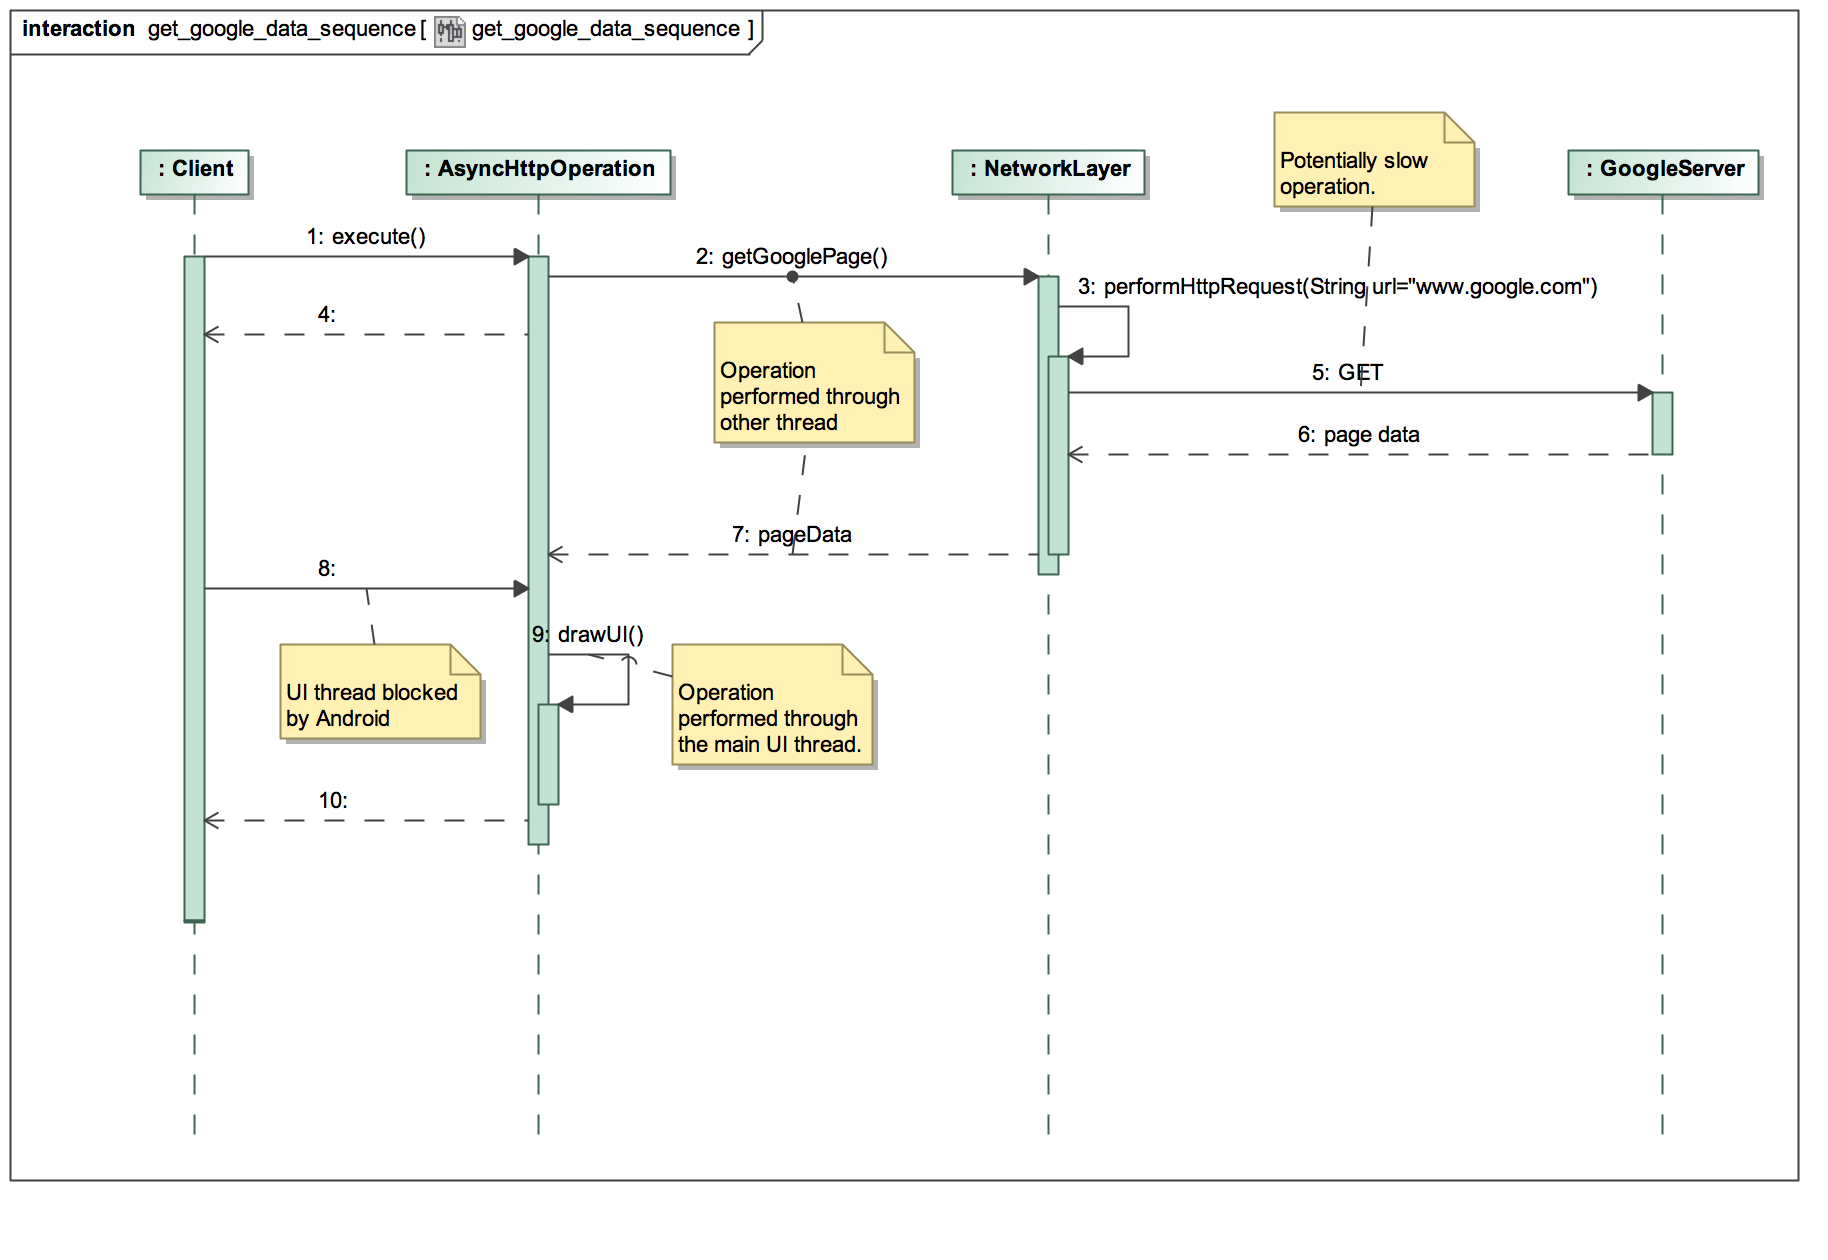
\includegraphics[scale=0.4]{../naive/design_models/get_google_data_sequence}
\end{center}
\end{figure}
\end{frame}

\begin{frame}{Explanation}
\begin{enumerate}
\item {\bf Main thread}: Once ``execute'' is called it returns the control inmediately.
\item {\bf Secondary thread}: Meanwhile, this thread does the http request and analizes the response.
\item {\bf Main thread}: Once the background job is finished, the main thread is blocked again and the UI actions are performed (for example, show a dialog or update a textview).
\end{enumerate}
\begin{itemize}
\item {\bf Note}: While the secondary thread performs the request, the main thread is able to execute any instructions (is usual to show a loading dialog).
\end{itemize}
\end{frame}

\subsection{Conclusions}
\begin{frame}{Conclusions}
\begin{itemize}
\item Whenever you need to make a request (a new or an already defined one but from another activity) and update the UI, you have to define a class that inherits from AsyncTask.
\item It's necessary to define the request to be performed (``NetworkOperationsManager'' class), the processing of the response and the UI update. Too many responsibilities.
\item There is too much coupling (it violates the SRP) $\rightarrow$ It is difficult to distribute the programming between UI and low-level (network operations and caches).
\end{itemize}
\end{frame}

\section{Second disgn: Callback-based}
\subsection{Callbacks}
\begin{frame}{What is a callback?}
\begin{itemize}
\item A callback is executable code that is passed as an argument to another code and is expected to be called at a given time.
\item There are two types of callbacks: blocking callbacks (also known as synchronous callbacks or just callbacks) and deferred callbacks (also known as asynchronous callbacks).
\item Deferred callbacks imply the existence of multiple threads.
\item They are a sort of ``Observer'' pattern.
\end{itemize}
\end{frame}

\begin{frame}[fragile]{Ejemplo de callback: Lectura de un fichero en Node.js}
\begin{lstlisting}
fs = require('fs');
fs.readFile('path', 'utf8', function(err,data) {
  if (err) {
    return console.log(err);
  }
  console.log(data);
});
\end{lstlisting}


\end{frame}

\subsection{Class diagram}
\begin{frame}
\begin{figure}
\begin{center}
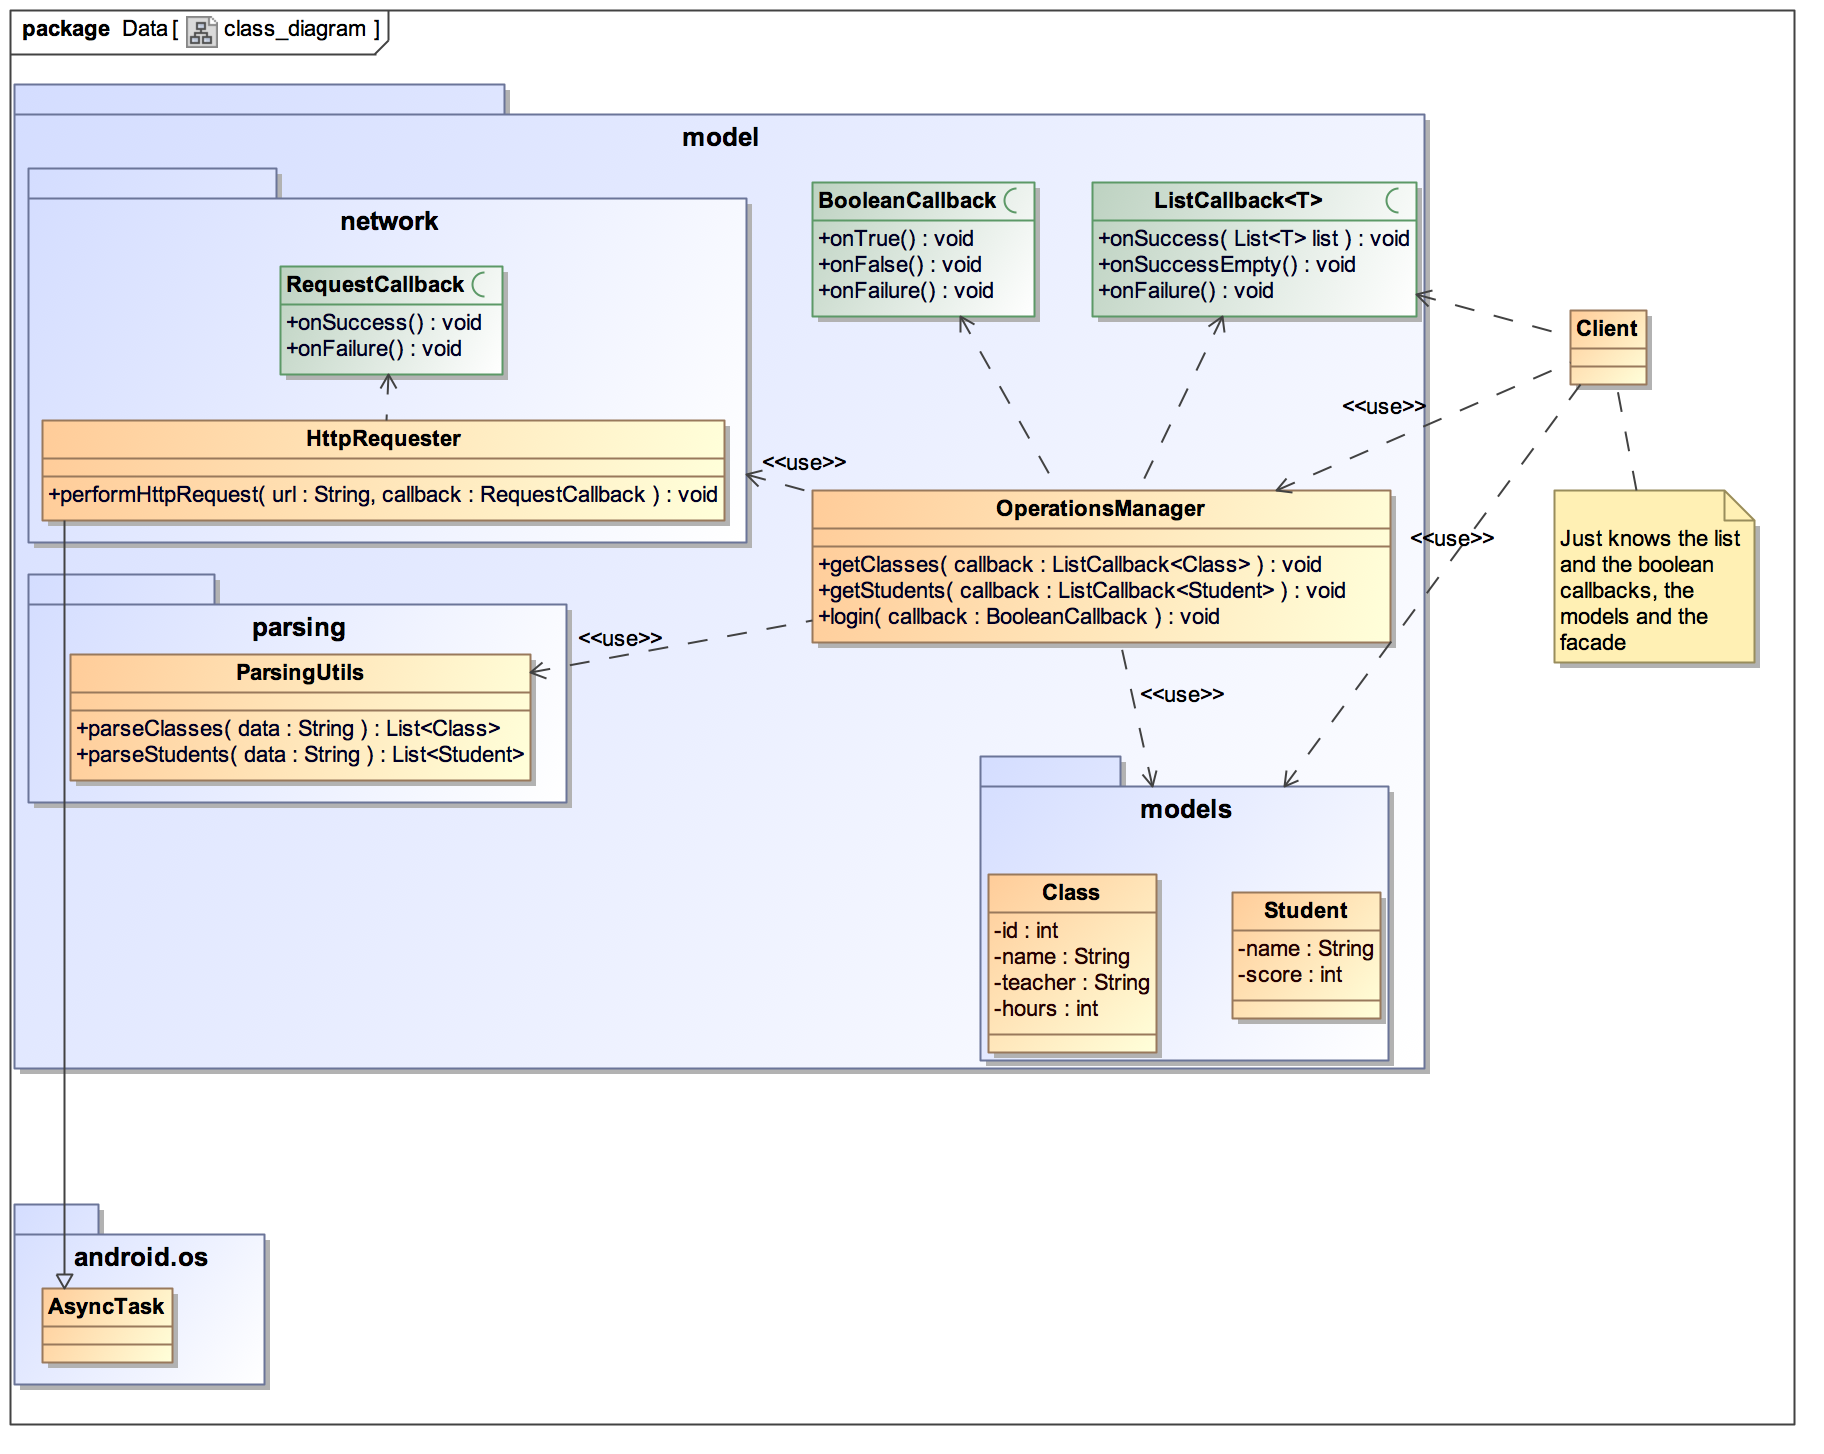
\includegraphics[scale=0.33]{../observer-pattern/diagrams/class_diagram}
\end{center}
\end{figure}
\end{frame}

\begin{frame}{Explanation (model inner layer)}
\begin{itemize}
\item {\bf Network}: This is the innermost package. It defines the basic action of making an HTTP request and ``doing something'' with the response. That ``something'' is defined by the ``requestCallback''.
\item {\bf Parsing}: Response parsing methods.
\end{itemize} 
\end{frame}

\begin{frame}{Explanation (model facade)}
\begin{itemize}
\item {\bf OperationsManager}: Entry point into the subsystem, provides network operations and requires callbacks for what to do with the answers.
\item {\bf Callbacks}: Different types of callbacks that may be required by the Operations Manager.
\item {\bf Value\_objects}: Classes that represent objects (equivalents to the ``C'' structs).
\end{itemize} 
\end{frame}

\subsection{Sequence diagram}
\begin{frame}
\begin{figure}
\begin{center}
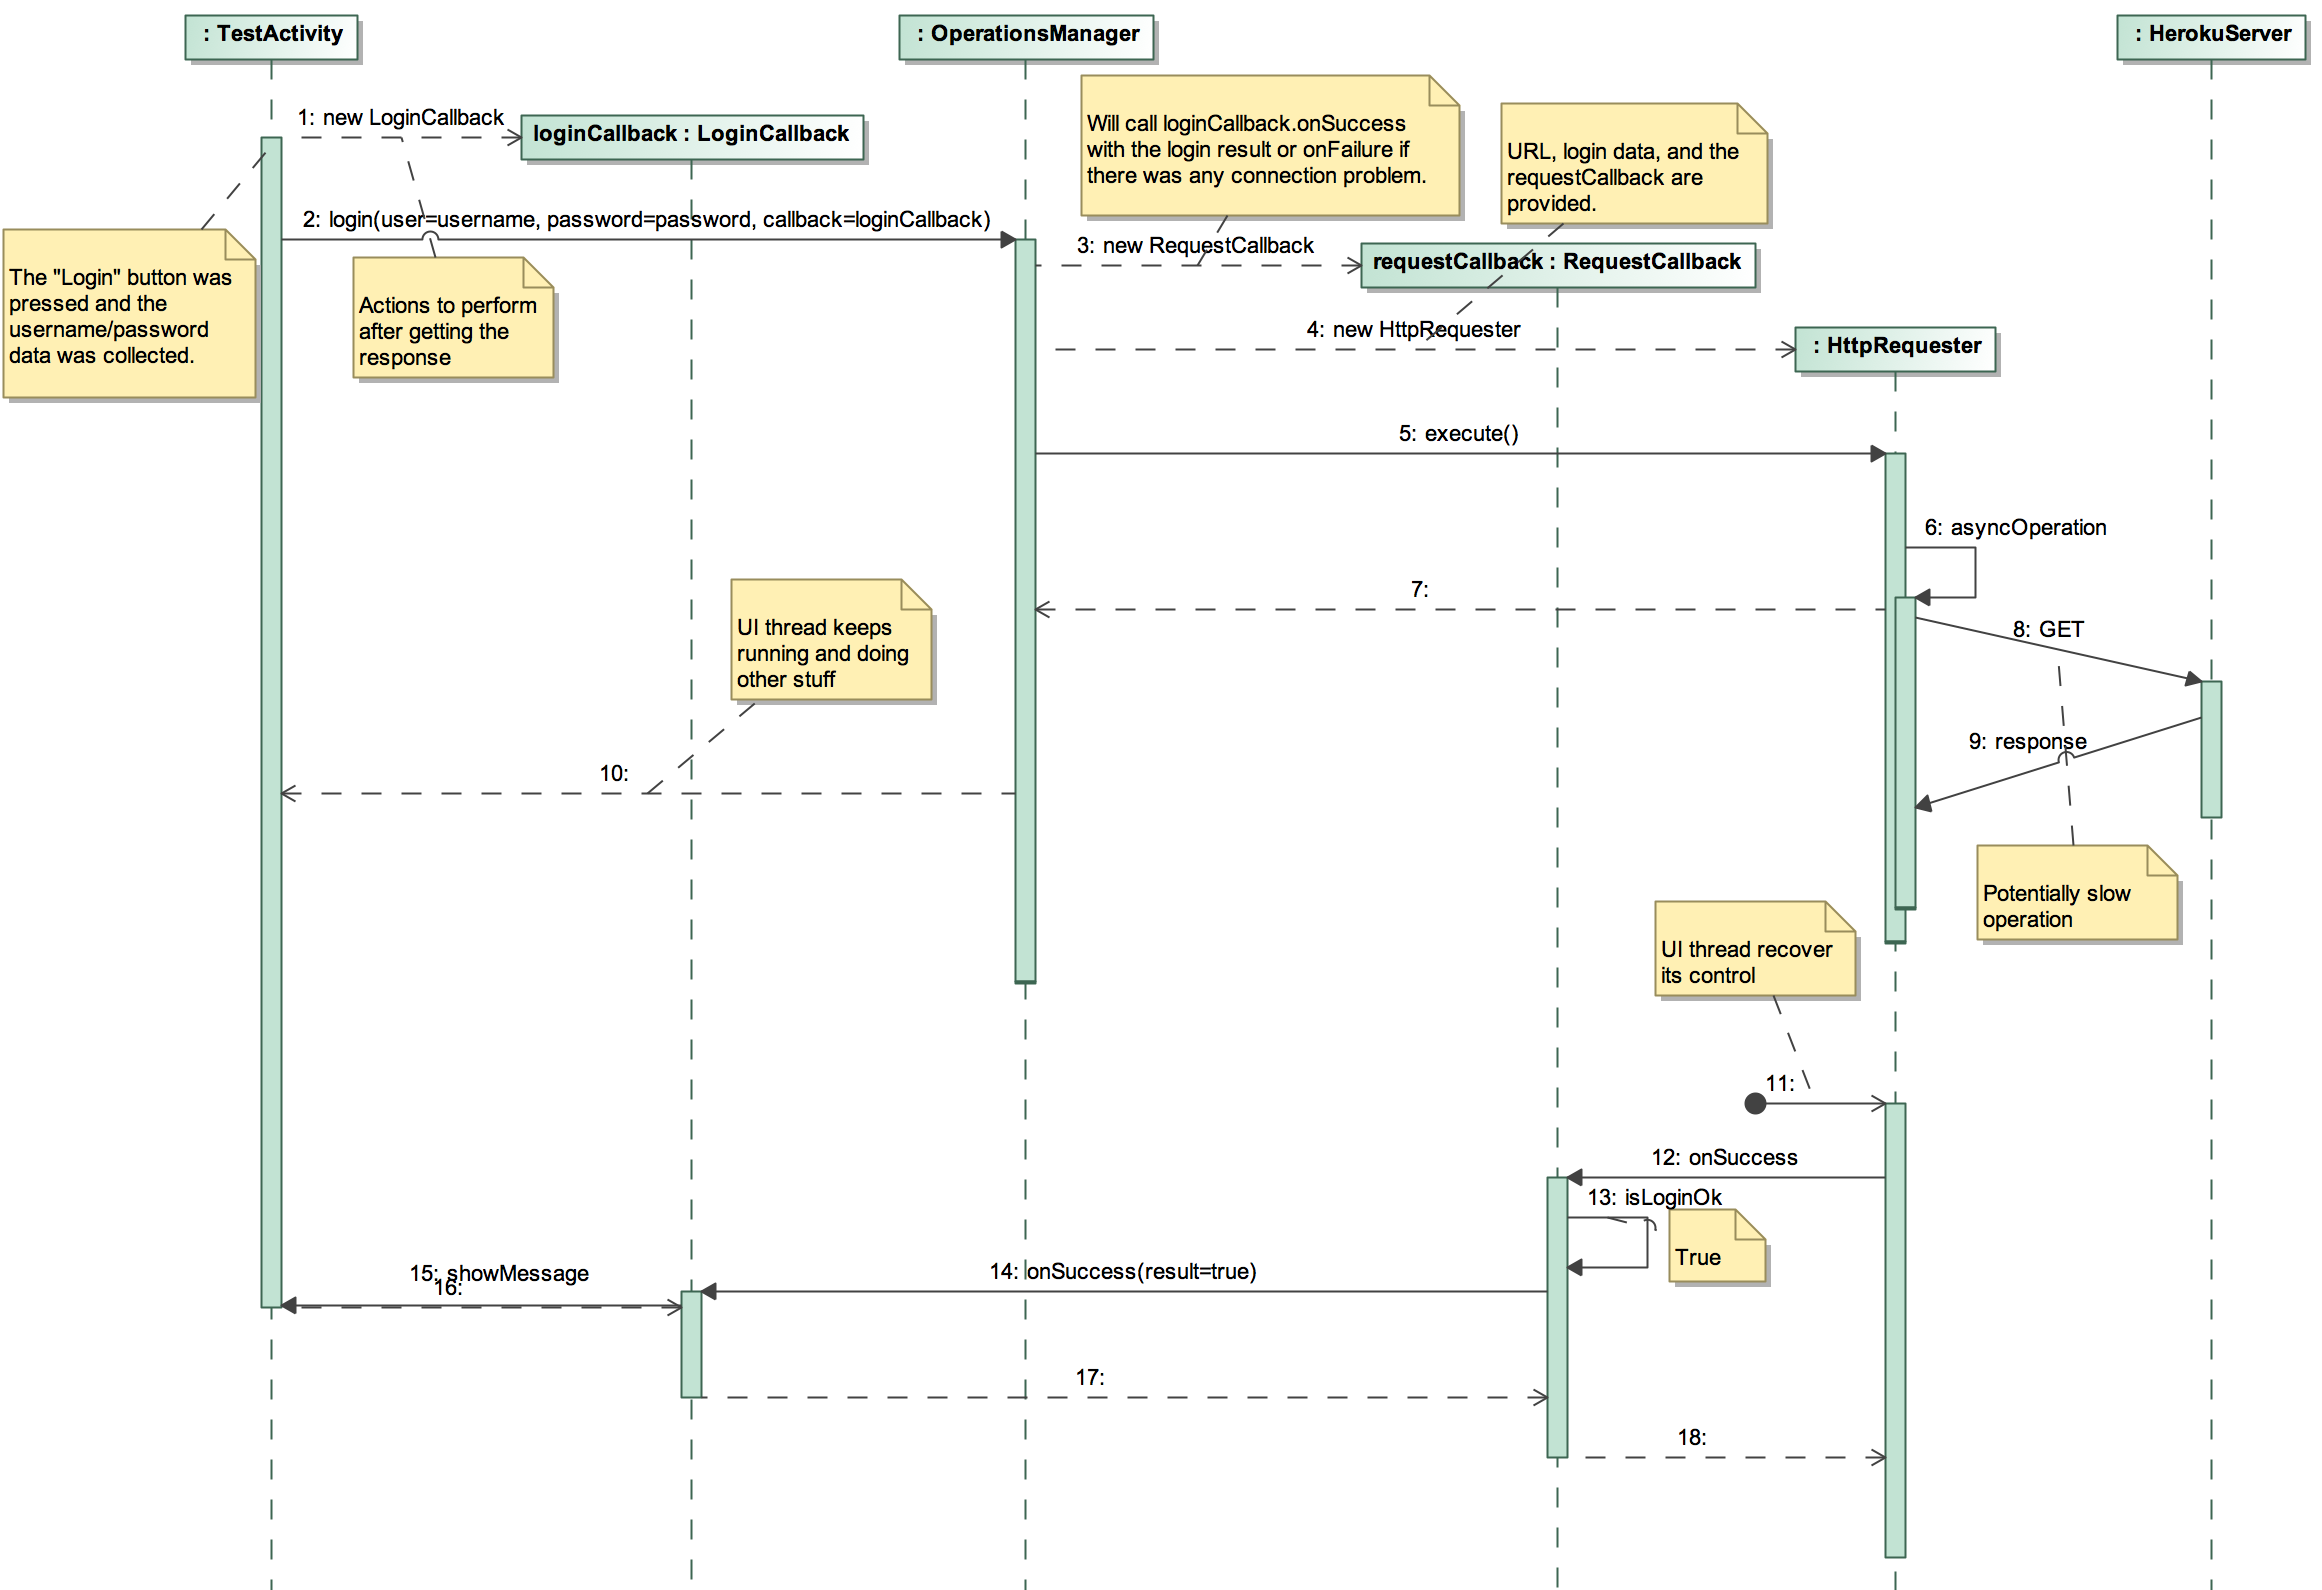
\includegraphics[scale=0.31]{../observer-pattern/diagrams/login}
\end{center}
\end{figure}
\end{frame}

\begin{frame}{Explanation}
\begin{enumerate}
\item It creates a LoginCallback (this class implements OperationCallback with the type Boolean as a parameter).
\item OperationsManager.getInstance().login(user, password, LoginCallback) is called.
\item Operations Manager creates a requestCallback and sends it to HttpRequester along with the address and request parameters.
\item Here begins the operation in the background. The UI thread is released.
\item When the operation is finished, it executes the requestCallback code.
\end{enumerate} 
\end{frame}
\subsection{Conclusions}
\begin{frame}[fragile]{Conclusions}
\begin{itemize}
\item This approach is based on three concepts: MVC architecture, Observer pattern (callbacks) and Facade pattern.
\item {\bf Advantages}:
\begin{itemize}

\item All the responsibilities are clearly separated.
\item The client only needs to know the facade of the network module.
\item his approach allows to divide the network and UI programming completely. Connecting them is straightforward.
\end{itemize}

\item {\bf Hándicaps}: 
\begin{itemize}
\item There is some repetition of code which cannot be generalized in the ``onFailure'' methods.
\item The alternative is to use an abstract class (but we could not implement the interface  directly into a `` Activity'' if it were simple enough).
\end{itemize}
\end{itemize}
\end{frame}

\section{Extra notes}
\begin{frame}{Extra}
\begin{itemize}
\item The innermost module is common to many Android apps $ \ rightarrow $ Turn it into a library.
\item Someone had the idea before and has done a very good job: {\url http://loopj.com/android-async-http/}
\item This same design can be applied to any other Java application (or other platform) as long as it implements a mechanism similar to AsyncTask (many platforms do not need to update the interface from the main thread).
\end{itemize}
\end{frame}
\end{document}
